\chapter{МАТЕРІАЛИ ТА МЕТОДИ ДОСЛІДЖЕННЯ}
\section{Клінічна характеристика пацієнтів із гепатобластомою}
Для вирішення поставлених задач нами проведено комплексне дослідження пацієнтів з гепатобластомою печінки, яких було прооперовано у відділенні трансплантації і хірургії печінки Національного інституту хірургії та трансплантології імені О.О. Шалімова за період із січня 2005 по січень 2020 р. Всього було прооперовано 90 дітей з гепатобластомою, з яких 81 пацієнту виконана резекція печінки, а в 9 випадках нерезектабельної гепатобластоми виконана трансплантація частини печінки від живого родинного донора. 

Розподілення пацієнтів за віком та статтю наведено у діаграмі (Рис. \ref{fig:mw})

% Please add the following required packages to your document preamble:
% \usepackage{graphicx}
% \usepackage[table,xcdraw]{xcolor}
% If you use beamer only pass "xcolor=table" option, i.e. \documentclass[xcolor=table]{beamer}
\begin{table}[]
\centering
\caption{Розподілення пацієнтів по статі.}
\label{tab:sex}
\begin{tabular}{|p{0.1\linewidth}|p{0.1\linewidth}|p{0.1\linewidth}|}
\hline
\textbf{Стать}    & {\color[HTML]{231F20} \textbf{Кількість}} & {\color[HTML]{231F20} \textbf{\%}} \\ \hline
\textbf{Чоловіча} & 59                                        & 65,5\%                            \\ \hline
\textbf{Жіноча}   & 31                                        & 34,4\%                            \\ \hline
\end{tabular}
\end{table}

Із 90 пацієнтів 59 було чоловічої статі та 31 жіночої (Таб. \ref{tab:sex}). 66 пацієнтів була віком до 3 років, що склало 76,7\%. Дітей віком до 1 року було всього 20, що склало 23,3\%; віком від 1 до 2 років 22, що склало 25,8\%; від 2 до 3 років – 24 пацієнта (27,9\%); 20 пацієнтів з 3 до 10 років, що склало 23,3\%.

В нашій работі ми використовували Брисбанську класификацію анатомії сегментів печінки та свідповідних резекцій печінки комітету Гепато-панкреато-біліарної Асоціації (2000 р.) \cite{pmid24852330}, яка базується на сегментарній будові печінки по C.Cuonoud. Класифікація базується на поділі печінки на секції, сектори та сегменти відповідно поділу портальних структур першого, другого та третього порядку. Згідно класифікації виділяють: 

\begin{itemize}
    \item Поділ першого порядку
    \begin{itemize}
    \item Ліва напівпечінка (Sg 2-4 ± Sg1 по C.Cuonoud), операція - лівобічна гемігепатектомія
    \item Права напівпечінка (Sg 5-8 ± Sg1 по C.Cuonoud), операція - правобічна гемігепатектмія
\end{itemize}
\end{itemize}
\begin{itemize}
    \item Поділ другого порядку
    \begin{itemize}
    \item Ліва латеральна секція (Sg 2-3 ± Sg1 по C.Cuonoud), операція - лівобічна латеральна секціоектомія
    \item Ліва медіальна секція (Sg 4 по C.Cuonoud), операція - лівобічна медіальна секціоектомія
    \item Права передня секція (Sg 5-8 по C.Cuonoud), операція - правобічна передня секціоектомія
    \item Права задня секція (Sg 6-7 по C.Cuonoud), операція - правобічна задня секціоектомія
\end{itemize}
\end{itemize}
    \begin{itemize}
    \item Поділ третього порядку
    \begin{itemize}
    \item Сегменти з 1-го по 9-й, операція - сегментектомія відповідних сегментів
    \item Два суміжних сегменти ((Sg 5-6, Sg 7-8, Sg 1-9), операція - бісегментектомія
\end{itemize}
\end{itemize}

Для резекцій 3 секцій печінки використовують назви лівобічна (Sg 2-5, Sg 8 ± Sg1 по C.Cuonoud) та правобічна  (Sg 4-8 ± Sg1 по C.Cuonoud) трисекціоектомії.

Пацієнти були оцінені за шкалою дохірургічної оцінки  гепатобластом у дітей PRETEXT (pre-treatment extent of disease) відповідно рекомендацій SIOPEL (Рис. \ref{fig:pretexpac}). За цією шкалою стадія PRETEXT визначається на підставі поширення пухлини на секції печінки за даними МРТ або КТ і включають наступні критерії: 
PRETEXT I – пухлина виявлена в межах однієї секції печінки; 
PRETEXT II – у двох секціях печінки; 
PRETEXT III – пухлина виявлена у трьох секціях печінки, вільна від пухлини тільки одна секція; 
PRETEXT IV – рак виявлений у всіх чотирьох секціях печінки. 

\begin{figure}[h]
\centering
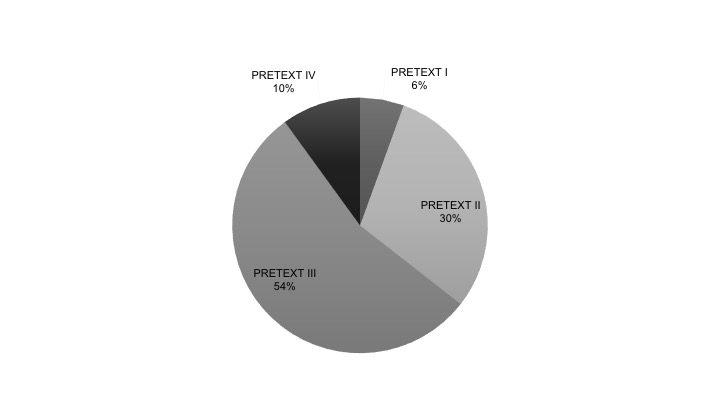
\includegraphics[width=0.7\textwidth]{Illustrations/pretexpac.jpeg}
\label{fig:pretexpac} % Назва малюнку
\caption{Розподіл пацієнтів за класифікацією PRETEXT.}
\end{figure}


Резекція печінки була виконана при гепатобластомі PRETEXT-I, II, III, як первинна резекція у 88 дітей, і в 2-х випадках при рецидивній гепатобластомі виконана ререзекція печінки. При нерезектабельній гепатобластомі PRETEXT-IV з пухлинним ураженням всіх секцій печінки і PRETEXT-III з настільки близьким розташуванням до судин воріт печінки або печінковим венам, що малоймовірно досягнути «tumor free margin» резекційної площини, при відсутності за даними КТ і МРТ віддалених метастазів, виконана трансплантація печінки у 9 випадках.

Згідно класифікації PRETEXT І стадію було встанолено у 5 пацієнтів, що відповідає 5,6\%, ІІ стадія у 27 пацієнтів – 30,0\%, ІІІ стадія у 49 пацієнтів – 54,4\%, та ІV стадія у 9 пацієнтів – 10,0\% (Рис. \ref{fig:pretexpac}).
(Таб. \ref{tab:pretexpvfc})
% Please add the following required packages to your document preamble:
% \usepackage{graphicx}
% \usepackage[table,xcdraw]{xcolor}
% If you use beamer only pass "xcolor=table" option, i.e. \documentclass[xcolor=table]{beamer}
\begin{table}[]
\centering
\caption{Розподілення пацієнтів по стадії PRETEXT }
\label{tab:pretexpvfc}
\resizebox{\textwidth}{!}{%
\begin{tabular}{|
>{\columncolor[HTML]{FFFFFF}}l |
>{\columncolor[HTML]{FFFFFF}}l |
>{\columncolor[HTML]{FFFFFF}}l |
>{\columncolor[HTML]{FFFFFF}}l |}
\hline
\textbf{} &
  {\color[HTML]{231F20} \textbf{Резекційна група (n=81)}} &
  {\color[HTML]{231F20} \textbf{Трансплантаційна група (n=9)}} &
  {\color[HTML]{231F20} \textbf{Значимість відмінностей, p}} \\ \hline
\textbf{PRETEXT I}                           & 5  & - & \textbf{0,03} \\ \hline
\textbf{PRETEXT IІ}                          & 27 & - & \textbf{0,04} \\ \hline
\textbf{PRETEXT IІІ}                         & 49 & - & \textbf{0,02} \\ \hline
\textbf{PRETEXT IV}                          & -  & 9 & \textbf{0,02} \\ \hline
\textbf{P (Інвазія в ворітну вену)}          & 3  & 5 & \textbf{0,03} \\ \hline
\textbf{V (Інвазія в печінкові вени, НПВ)}   & 9  & 6 & \textbf{0,04} \\ \hline
\textbf{F (Мультифокальна пухлина)}          & 56 & 9 & \textbf{0,02} \\ \hline
\textbf{С (Поширення на SgI)}                & 49 & 8 & \textbf{0,02} \\ \hline
\textbf{E (Позапечінкове поширення пухлини)} & 3  & 1 & \textbf{0,03} \\ \hline
\textbf{R (Спонтанний розрив пухлини)}       & 5  & 3 & \textbf{0,04} \\ \hline
\textbf{M (Віддалені метастази)}             & 0  & 0 & \textbf{0,02} \\ \hline
\textbf{Інвазія в жовчні протоки}            & 1  & 5 & \textbf{0,02} \\ \hline
\end{tabular}%
}
\end{table}

В стандартний доопераційний протокол обстеження крім СКТ та МРТ також обов’язково входили загальний та біохімічний аналіз крові, коагулограма, визначення рівня альфа-фетопротеїну (АФП). У таблиці наведено основні показниками показники, які характеризують пацієнтів  з гепатобластомами у двох групах: резекційна та трансплантаційній групах. Статистично значущих відмінностей між групами не виявлено, крім одного критерію – рефрактерність до хіміотерапії була значно вищою у трансплантаційній групі (Таб. \ref{tab:haracter}). Це пов’язано, передусім, з тим, що у трансплантаційній групі у 78\% випадках при патогістологічному аналізі спостерігався змішаний епітеліально-мезенхімальний тип гепатобластоми, як правило, нечутливий до хіміотерапії. 

% Please add the following required packages to your document preamble:
% \usepackage{graphicx}
% \usepackage[table,xcdraw]{xcolor}
% If you use beamer only pass "xcolor=table" option, i.e. \documentclass[xcolor=table]{beamer}
\begin{table}[]
\centering
\caption{Основні характеристики резекційної та трансплантаційної груп пацієнтів із гепатобластомою}
\label{tab:haracter}
\resizebox{\textwidth}{!}{%
\begin{tabular}{|
>{\columncolor[HTML]{FFFFFF}}l |
>{\columncolor[HTML]{FFFFFF}}l |
>{\columncolor[HTML]{FFFFFF}}l |
>{\columncolor[HTML]{FFFFFF}}l |}
\hline
\textbf{Xapaктepнcтнкa} &
  {\color[HTML]{231F20} \textbf{Peзeкційнa rpyпa (n=81)}} &
  {\color[HTML]{231F20} \textbf{Tpaнcплaнтaційнa rpyпa (n=9)}} &
  {\color[HTML]{231F20} \textbf{P}} \\ \hline
{\color[HTML]{231F20} \textit{\textbf{Biк, мic.}}} &
  {\color[HTML]{231F20} \textbf{28 (6-59)}} &
  {\color[HTML]{231F20} \textbf{39 (8-66)}} &
  {\color[HTML]{231F20} \textbf{0,65}} \\ \hline
{\color[HTML]{231F20} \textit{\textbf{Cтaть (ч/ж)}}} &
  {\color[HTML]{231F20} 58/23} &
  {\color[HTML]{231F20} 6.3} &
  {\color[HTML]{231F20} 0,84} \\ \hline
{\color[HTML]{231F20} \textit{\textbf{Heoaд’ювaнтнa xiмioтepaпiя, n (\%)}}} &
  {\color[HTML]{231F20} 65 (80\%)} &
  {\color[HTML]{231F20} 9 (100\%)} &
  {\color[HTML]{231F20} 0,2} \\ \hline
{\color[HTML]{231F20} \textit{\textbf{AFP ≥ 100 ng/ml, n (\%)}}} &
  {\color[HTML]{231F20} 60 (74\%)} &
  {\color[HTML]{231F20} 9 (100\%)} &
  {\color[HTML]{231F20} 0,18} \\ \hline
\textbf{Позaпeчiнкoвi мeтacтaзи, n(\%)}         & 4 (7\%)     & −          & 0,48   \\ \hline
\textbf{Бiлipyбiн (mmol/l)}                     & 24,7±7,2    & 28,3±9,5   & 0,56   \\ \hline
\textbf{ACT (U/L)}                              & 52,7±7,4    & 65,2±8,6   & 0,74   \\ \hline
\textbf{AЛT (U/L)}                              & 67,6±6,3    & 76,4±7,3   & 0,76   \\ \hline
\textbf{Пpoтpoмбінoвий чac, c}                  & 17,6±1,2    & 18,5±2,5   & 0,85   \\ \hline
\textbf{Peфpaктepнicть дo xiмioтepaпiï, n (\%)} & 20 (24,7\%) & 5 (66,6\%) & 0,034* \\ \hline
\end{tabular}%
}
\end{table}

Основна частина пацієнтів була з верифікованими патогістологічними діагнозами після обов'язкової біопсії пухлини, за винятком 12 випадків (14,8\%) гепатобластоми PRETEXT I-II, коли виконана первинна резекція печінки без неоад’ювантної ХТ.
Для визначення алгоритму лікування гепатобластоми пацієнти були стратифіковані на групи ризику по системі Children’s Hepatic tumors International Collaboration—Hepatoblastoma Stratification (CHIC-HS) на основі найбільш прогностичних діагностичних факторів, які виявились при первинному аналізі: 

\begin{itemize}
    \item стадія PRETEXT; 
    \item вік молодший 3 років, 3–7 років та 8 років або старше;
    \item концентрація альфафетопротеїну (AFP) 100 нг/мл або нижче і 101-1000 нг/мл;
    \item наявність або відсутність метастазів;
    \item аявність або відсутність «VPEFR» : макроваскулярного ураження всіх печінкових вен (V) або портальної біфуркації (P), суміжної позапечінкової пухлини (E), мультифокальної пухлини (F) та спонтанного розриву пухлини (R).
\end{itemize}

При оцінці стану пацієнтів по системі CHICS було встановлено, що у 50 (55,6\%) пацієнтів був середній ризик за цією шкалою, у 24 (26,7\%) високий ризик, і у 16 (17,8\%) пацієнтів був дуже високий ризик  (Таб. \ref{tab:CHICS}). Питома вага пацієнтів з високим та дуже високим ступенем ризику був вищим у групі пацієнтів, яким виконали трансплантацію печінки в порівнянні з пацієнтами з резекціями печінки.





% Please add the following required packages to your document preamble:
% \usepackage{graphicx}
% \usepackage[table,xcdraw]{xcolor}
% If you use beamer only pass "xcolor=table" option, i.e. \documentclass[xcolor=table]{beamer}
\begin{table}[]
\centering
\caption{Розподіл пацієнтів по групах ризику гепатобластом по системі CHICS (Children’s Hepatic Tumors International Collaboration`s Stratification)}
\label{tab:CHICS}
\resizebox{\textwidth}{!}{%
\begin{tabular}{|
>{\columncolor[HTML]{FFFFFF}}l |
>{\columncolor[HTML]{FFFFFF}}l 
>{\columncolor[HTML]{FFFFFF}}l |
>{\columncolor[HTML]{FFFFFF}}l 
>{\columncolor[HTML]{FFFFFF}}l |
>{\columncolor[HTML]{FFFFFF}}l 
>{\columncolor[HTML]{FFFFFF}}l |}
\hline
\textbf{Групи ризику} &
  \multicolumn{2}{l|}{\cellcolor[HTML]{FFFFFF}{\color[HTML]{231F20} \textbf{Резекційна група}}} &
  \multicolumn{2}{l|}{\cellcolor[HTML]{FFFFFF}{\color[HTML]{231F20} \textbf{Трансплантаційна група}}} &
  \multicolumn{2}{l|}{\cellcolor[HTML]{FFFFFF}\textbf{Разом}} \\ \hline
{\color[HTML]{231F20} \textit{\textbf{Середній ризик (IR)}}} &
  \multicolumn{1}{l|}{\cellcolor[HTML]{FFFFFF}{\color[HTML]{231F20} \textbf{50}}} &
  {\color[HTML]{231F20} \textbf{61,70\%}} &
  \multicolumn{1}{l|}{\cellcolor[HTML]{FFFFFF}{\color[HTML]{231F20} \textbf{-}}} &
  {\color[HTML]{231F20} \textbf{-}} &
  \multicolumn{1}{l|}{\cellcolor[HTML]{FFFFFF}50} &
  55,60\% \\ \hline
{\color[HTML]{231F20} \textit{\textbf{Високий ризик (HR)}}} &
  \multicolumn{1}{l|}{\cellcolor[HTML]{FFFFFF}{\color[HTML]{231F20} 20}} &
  {\color[HTML]{231F20} 24,70\%} &
  \multicolumn{1}{l|}{\cellcolor[HTML]{FFFFFF}{\color[HTML]{231F20} 4}} &
  {\color[HTML]{231F20} 44,40\%} &
  \multicolumn{1}{l|}{\cellcolor[HTML]{FFFFFF}24} &
  26,70\% \\ \hline
{\color[HTML]{231F20} \textit{\textbf{Дуже високий ризик (VHR)}}} &
  \multicolumn{1}{l|}{\cellcolor[HTML]{FFFFFF}{\color[HTML]{231F20} 11}} &
  {\color[HTML]{231F20} 13,60\%} &
  \multicolumn{1}{l|}{\cellcolor[HTML]{FFFFFF}{\color[HTML]{231F20} 5}} &
  {\color[HTML]{231F20} 55,60\%} &
  \multicolumn{1}{l|}{\cellcolor[HTML]{FFFFFF}16} &
  17,80\% \\ \hline
{\color[HTML]{231F20} \textit{\textbf{Разом}}} &
  \multicolumn{1}{l|}{\cellcolor[HTML]{FFFFFF}{\color[HTML]{231F20} 81}} &
  {\color[HTML]{231F20} } &
  \multicolumn{1}{l|}{\cellcolor[HTML]{FFFFFF}{\color[HTML]{231F20} 9}} &
  {\color[HTML]{231F20} } &
  \multicolumn{1}{l|}{\cellcolor[HTML]{FFFFFF}90} &
   \\ \hline
\end{tabular}%
}
\end{table}


\section{Клінічна характеристика донорів}
Згідно Закону України про трсплантацію органів та інших анатомічних матеріалів людини (№1007-XIV від 16.07.1999), та Закону України про застосування трансплантації анатомічних матеріалів від (№ 2427-VII  17.05.2018) ми обстежували близьких родичів реципієнтів, які виявили добровільне бажання стати донором частини печінки. Згода донорів та їх родинні зв'язки з реципієнтом підтвердджено документально. 

Родинні зв'язки донора та реципієнта представлені в таблиці. Найчастіше в 6 випадках (66,6\%) це була матір пацієнта, і в 3 (33,3\%) - батько пацієнта. 
Всі донори були фізично та психологідно здоровими, не мали хронічної патології, інфекційних захворювань, що передаються трансмісивним шляхом. В 7 випадках реципієнт та донор мали однакову групу крові, у 2 - сумісну. Потенційним донорам, що несумісні по групах крові відмовляли в можливості доновання. Вікові обмеження для донорів складали 18-55 рокців. 
Шість пацієнтів (66,6\%) були жіночої статі, троє (33,3\%) - чоловічої. Середній вік донорів склав 31,9±9,3 роки. 
Судинну анатомію вивчали за допомогою СКТ з внутрішньовенним контрастуванням до операції. При чому вивчали судинну анатомію ворітноїх та печінкової вени а також печінкової артерії. 
За допомогою СКТ проводили волюметрію майбутнього трансплантата. 

\section{Методи дослідження}
\subsection{Алгоритм доопераційного обстеження}

Всім пацієнтам з гепатобластомою проведено комплексне обстеження, що включає клінічні, інструментальні та спеціальні методи дослідження.
Діагностичний алгоритм включав наступні завдання:
\begin{enumerate}
    \item установлення діагнозу гепатобластома;
    \item диференціальна діагностика з доброякісними пухлинами;
    \item визначення рівня ураження жовчного дерева;
    \item вивчення судинної анатомії портальних і кавальних воріт печінки;
    \item виявлення інвазії пухлини в воротну вену та печінкову артерію;
    \item виявлення віддалених метастазів;
    \item виявлення ураження регіональних лімфовузлів;
    \item визначення маси перспективного печінкового залишку;
    \item цінка функціонального стану печінки;
\end{enumerate}

Обстеження починали зі збору клініко-анамнестичних даних. У пацієнтів з перихілярною холангіокарциномою брали до уваги на скарги, наявність жовтяниці, температурну реакцію, перенесені оперативні втручання, супутню патологію, а також дані сімейного анамнезу. Наступним етапом проводили загально клінічні дослідження, що включає загальний аналіз крові з лейкоцитарною формулою, загальний аналіз сечі, біохімічне дослідження крові, коагулограму. Також визначали онкомаркери Са 19-9, альфафетопротеїн, раково-ембріональний антиген. З метою виявлення супутнього вірусного гепатиту визначали маркери вірусних гепатитів В і С.

\begin{figure}[h]
\centering
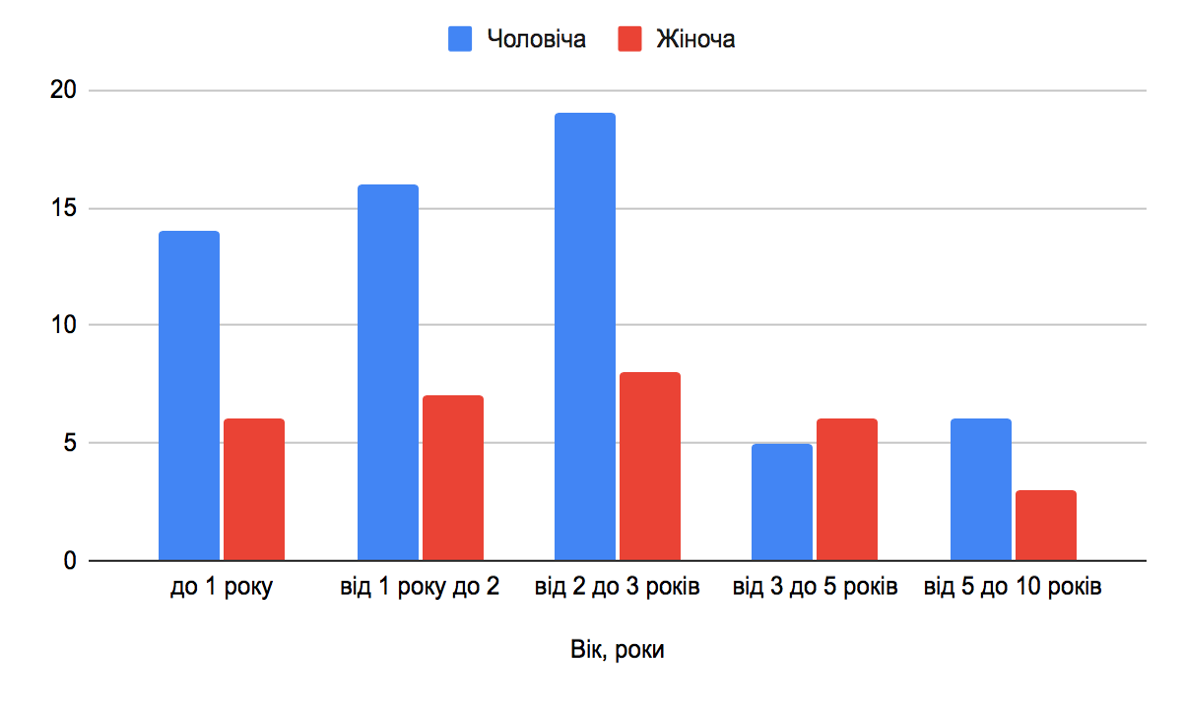
\includegraphics[width=0.7\textwidth]{Illustrations/mw.png}
\label{fig:mw} % Назва малюнку
\caption{Розподілення пацієнтів за віком та статтю.}
\end{figure}

З інструментальних досліджень всім хворим в обов'язковому порядку виконували спіральну комп'ютерну томографію органів черевної порожнини і грудної клітки, магнітно-резонансна томографія, МРТ-холангіографію, УЗД черевної порожнини, УЗДС портальної системи і судин печінки, ЕКГ, ЕхоКГ, ФЕГДС і колоноскопію. 

Для вивчення судинної анатомії портальних і кавальних воріт печінки, виявлення інвазії пухлини в воротну вену, печінкову артерію, наявності метастазування в регіональні лімфатичні вузли і віддалені органи виконували СКТ органів черевної порожнини і грудної клітки з внутрішньовенним підсиленням. Використовували спіральний комп'ютерний томограф LightSpeed-16 фірми General Electric c шириною зрізу 5 мм. Методику виконували наступним чином. Контрастування вісцеральних судин здійснювали за допомогою внутрішньовенного введення контрасту «Омніпак», в дозі 5 мл на 1 кг. ваги, але не більше 300 мл. Час за яке контраст досягав печінкової артерії склало в середньому 18-27 секунд а печінкових вен - 50-80 секунд. Отримані зрізи обробляли і перетворювали в 3-х мірне зображення судинного русла. Для оцінки ступеня гепатоза печінки хворого, порівнювали денситометричну щільність печінки та селезінки.

За допомогою СКТ проводили волюметр перспективного печінкового залишку печінки і обсяг планованого видаляється частини печінки. Для виконання волюметр печінки виконували роздруківку на плівці послідовних КТ-зрізів паренхиматозний фази виведення контрасту починаючи від рівня правого купола діафрагми і включаючи всі зрізи із зображенням печінки. Всі зрізи друкували з одним і тим же збільшенням, а на одному зі зрізів вказували лінійку масштабу, що відповідає 10 см.

\[ V = 100 * \frac{\sum_{} (S)}{l^2}*h \]
де 
V - об'єм вимірюваного сегмента печінки в см$^3$
Σ (S) - сума площ всіх зрізів вимірюваного сегмента печінки в пікселах
l - довжина масштабної 10-сантиметрової лінійки в пікселах
h - інтервал між зрізами томографа в сантиметрах

Магнітно-резонансну томографію та МРТ холангіографію виконували з метою візуалізації рівня ураження жовчного дерева, інвазії пухлини в вісцеральні судини і метастатичне ураження лімфатичних вузлів.  Дослідження виконували на магнітно-резонасном томографі Siemens Magnetom Avanto 1,5 тесла, c використанням внутрішньовенного контрасту «Магневіст». Метод МРТ дифузії печінки дозволяє диференціювати доброякісні та злоякісні стриктури жовчних протоків. Зображення, одержувані в ході МРТ холангіографії, дозволяють оцінити поширення пухлини вздовж жовчних протоків та визначити тип поразки згідно класифікації Bismuth-Corlette. Це ключове дослідження для визначення резектабельності та планування об'єму резекції печінки.

Ультразвукове дослідження органів черевної порожнини проводили всім пацієнтам за допомогою УЗ сканерів SSD 120 і SSD 256 фірми «Aloka» з конвексним датчиком частотою 3,5-5,0 МГц для дослідження стану печінки, виявлення розширення жовчних протоків, рівня блоку жовчних протоків, розмірів селезінки, виявлення асциту та інших рідинних скупчень, анатомічних взаємовідносин органів, виявлення супутньої патології.

УЗДС судин печінки виробляли з метою первинного вивчення анатомії внутрішньопечінкових судин і судин портальної системи в передопераційному періоді та подальшого післяопераційного контролю кровотоку в печінковому залишку. Всіх хворих досліджували вранці, натщесерце. Дослідження проводилося на сканері «Tehnos» МРХ (ESACOTE SPA – Італія), з використанням конвексного датчика частотою 3,5-5,0 МГц. Застосовувалися режими сіро-шкального сканування, колірного і енергетичного допплерівського картування, імпульсно-хвильової доплерографії та їх різні комбінації. Дослідження починали в положенні хворого лежачи на спині через трансабдомінальний доступ з частотою датчика 5,0 МГц. Наступним етапом виконували черезреберне сканування в положенні хворого на спині, при необхідності використовували поворот хворого на лівий бік. Використовували сагітальній, горизонтальне і косе сканування з метою візуалізації стовбура воротної вени та її гілок, власної печінкової артерії і її гілок, системи печінкових вен і НПВ. При неадекватній візуалізації частоту датчика зменшували до 3,5 МГц.

Кольорове допплерівське сканування здійснювали з використанням швидкісної шкали середньої швидкості кровотоку 8-12 см / с при величині частоти повторення імпульсів 750-1000 Гц. При виявленні сигналів кровотоку використовували режим іпульснохвильової спектральної доплерографії, контрольний обсяг якої вибирали відповідно до діаметру судини (контрольний обсяг становив приблизно дві третини діаметра). В артеріальних судинах при реєстрації спектру кровотоку оцінювали максимальну лінійну систолічну (пікову) швидкість, індекс опору. Індекс резистентності розраховували як відношення різниці лінійної систолічної та діастолічної швидкостей до лінійної систолічної швидкості кровотоку. Індекс дозволяє оцінити судинний опір судинного русла. У венозних судинах оцінювали максимальну швидкість кровотоку усереднену за часом (TAV) і об'ємну швидкість кровотоку.

\subsection{Алгоритм післяопераційного обстеження}

Діагностичний алгоритм в післяопераційному періоді включав наступні завдання:

\begin{enumerate}
    \item морфологічне дослідження;
    \begin{enumerate}
    \item верифікація гістологічного типу пухлини;
    \item визначення чистоти резекційну краю;
    \item визначення типу гепатобластоми
    \item визначення ураження регіональних лімфатичних вузлів;
\end{enumerate}
    \item дослідження портального кровотоку в досліджуваній групі;
    \item оцінка функціонального стану печінки в післяопераційному періоді;
    \item оцінка післяопераційних ускладнень;
    \item оцінка віддаленій виживаності пацієнтів з гепатобластомою;
\end{enumerate}






Гістологічне дослідження здійснювали всім пацієнтам основної групи та групи порівняння. Операційний матеріал фіксували в 10\% нейтральному формаліні, гістологічні зрізи, отримані після стандартної гістологічної обробки, фарбували гематоксиліном-еозином, Азуро II- еозином по Ван Гізон. Досліджували зону пухлини, дистальний і проксимальні відділи жовчного дерева, лімфатичні вузли, а в досліджуваній групі і стінку воротної вени.

У ранньому післяопераційному періоді для оцінки функціонального стану печінки оцінювали загальний аналіз крові, розгорнутий біохімічний аналіз крові і показники коагулограми на 1, 3, 7, 10 добу. У досліджуваній групі на 1, 3, 7, 10 виконували оцінку портального кровотоку за допомогою УЗДГ. При наявності показань в післяопераційному періоді виконували спіральну комп'ютерну томографію, рентгенографію органів грудної клітини, оглядову рентгенографію органів черевної порожнини рентген або КТ холангіоргафію.  

Для оцінки важкості ускладнень в післяопераційному періоді використовували класифікацію Dindo - Clavien (табл.). Згодної цієї класифікації, визначали ступінь тяжкості кожного ускладнення
Для оцінки стану печінки і виявлення віддалених ускладнень і рецидиву, пацієнти проходили планове обстеження. У віддаленому післяопераційному періоді оцінювали загальний аналіз крові, біохімічний аналіз крові, коагулограму, онкомаркер АФП, спіральну комп'ютерну томографію органів черевної порожнини і грудної клітки і при наявності показань МРТ і МРТ холангіографія. Періодичність контролю в віддаленому післяопераційному періоді склала кожні 3 місяці протягом першого року і далі 1 раз на рік.

Таблиця - Класифікація ускладнень по Dindo - Clavien 


Статистичну обробку результатів здійснювали з використанням програмного пакету SPSS 20. Метод статистичного аналізу вибирали на підставі розподілу даних. Достовірними вважали результати тестів з рівнем значущості p<0,05. Відповідність розподілу досліджуваної вибірки нормальному визначали за допомогою тесту Шапіро-Уілкі. У всіх вибірках нами виявлено розподіл відмінне від нормального.

Для порівняння показників в групах використовували непараметричні критерії для незалежних вибірок - тести Круськала-Уолліса, при виявленні статистично значущих відмінностей результат перевіряли за допомогою тесту Манна-Уїтні. При цьому післяопераційний період поділяли на категорії (до операції, 0-добу, 1 добу, 3 добу, 7 добу, 10 добу, віддалений період), а потім виконували порівняння груп для кожної категорії. Для вивчення значущості відмінностей зміни лабораторних показників в часі використовували непараметричний аналог дисперсного аналізу - критерій Фрідмана. При виявленні статистично значущих результатів виконували перевірку за допомогою непараметричного тесту Вілкоксона для пов'язаних вибірок між сусідніми категоріями. Для аналізу виживаності будували криву Каплана-Мейера, порівняння виживання в групах оцінювали за допомогою Log-rank критерію. Для виявлення предикторів виживання застосовували мультифакторна регресію Кокса, а для виявлення впливу вихідних даних реципієнта на летальність, тяжкість і кількість ускладнень застосовували лінійну регресійну модель. Ускладнення і ранню післяопераційну летальність протягом 30 днів порівнювали за допомогою тесту Хі-квадрат




Ретроспективно проаналізовані такі показники, як тривалість операції, об’єм інтраопераційної кровотечі, терміни перебування у відділенні інтенсивної терапії та госпіталізації, ускладнення за класифікацією Clavien-Dindo і післяопераційна летальність в залежності від об’єму резекції печінки і складності операції, морбідность і виживаність (загальна і безрецидивна). 

В післяопераційному періоді моніторинг і регулярні спостереження включали: визначення рівня АФП в крові, КТ органів черевної і грудної порожнин, загальноклінічні і біохімічні аналізи крові, і проводились 4 рази в перший рік після операції, 3 раза на протязі 2-го року після операції, 2 раза на 3-му року. Після 3-х років після операції контрольні обстеження проводились 1 раз на рік на протязі 5 років. В разі виникнення рецидиву гепатобластоми в печінці, розглядалася повторна резекція печінки або трансплантація печінки.



Нами був розроблений алгоритм обстеження і передоперационої підготовки хворих з гепатобластомою.
При оцінці показників загального аналізу крові, що включають гемоглобін, еритроцити, лейкоцити, тромбоцити, в досліджуваній групі і групі порівняння, не виявлено статистично значущої різниці.

Показники біохімічного аналізу крові, що включають в себе показники загального та прямого білірубіну, загального білку, альбуміну, аланінамінотрансферази (АЛТ), аспартатамінотрансферази (АСТ), гамма-глютаматтрпнсфераза (ГГТП), лужної фосфатази (ЛФ) і лактатдегідрогенази (ЛДГ) були однорідни в обох групах.

Оцінка показників коагулограми показала статистично значущу різницю міжнародного нормалізованого відношення (INR) і активованого часткового тромбопластичного часу (АЧТЧ) (p = 0,03 критерій Манна-Уїтні), а різниця показників протромбінового часу і індексу статистично незначущі. 


